% This is LLNCS.DEM the demonstration file of
% the LaTeX macro package from Springer-Verlag
% for Lecture Notes in Computer Science,
% version 2.4 for LaTeX2e as of 16. April 2010
%
\documentclass{llncs}
\usepackage{algorithm}
\usepackage{algorithmic}
\usepackage{epsfig}
\usepackage{graphicx}
\usepackage{xcolor}
\usepackage{amsfonts,amsmath,amssymb}
\usepackage{fixltx2e} % Fixing numbering problem when using figure/table* 
\usepackage{subfig}
\usepackage{tabularx,ragged2e,booktabs}
\usepackage{float}
%\restylefloat{figure}
%\restylefloat{table}
\usepackage{todonotes}
\usepackage{makeidx}  % allows for indexgeneration
%
\newcolumntype{C}[1]{>{\Centering}m{#1}}
\renewcommand\tabularxcolumn[1]{C{#1}}
\setlength{\parindent}{10pt}
\renewcommand{\tablename}{\bf Table}
%
%% Package to linebreak URLs in a sane manner.
\usepackage{url}
%% Define a new 'smallurl' style for the package that will use a smaller font.
\makeatletter
\def\url@smallurlstyle{%
  \@ifundefined{selectfont}{\def\UrlFont{\sf}}{\def\UrlFont{\small\ttfamily}}}
\makeatother
%% Now actually use the newly defined style.
\urlstyle{smallurl}
%% Define 'tinyurl' style for even smaller URLs (such as in tables)
\makeatletter
\def\url@tinyurlstyle{%
  \@ifundefined{selectfont}{\def\UrlFont{\sf}}{\def\UrlFont{\scriptsize\ttfamily}}}
\makeatother
%
\begin{document}
%
\mainmatter              % start of the contributions
%
\title{SAX-VSM: \\Time Series Classification Using SAX Representation and Vector Space Model.}
%
\titlerunning{Timeseries features discovery with SAX and TF-IDF weighting}  
% abbreviated title (forrunning head)
%                                     also used for the TOC unless
%                                     \toctitle is used
%
\author{Pavel Senin\inst{1}
\and Sergey Malinchik\inst{2}
}
%
\authorrunning{Pavel Senin} % abbreviated author list (for running head)
%
%%%% list of authors for the TOC (use if author list has to be modified)
%\tocauthor{Ivar Ekeland, Roger Temam, Jeffrey Dean, David Grove,
%Craig Chambers, Kim B. Bruce, and Elisa Bertino}
%
\institute{Collaborative Software Development Laboratory,\\
Information and Computer Sciences Department,\\
University of Hawaii at Manoa,\\ Honolulu HI 96822, USA,\\
\email{senin@hawaii.edu}
\and
Lockheed Martin Advanced Technology Laboratories,\\
3 Executive Campus, Suite 600, Cherry Hill, NJ 08002, USA,\\
\email{sergey.b.malinchik@lmco.com}}


\maketitle              % typeset the title of the contribution

\begin{abstract}
Ability to discover characteristic patterns in time series paves the road for many
downstream analyses while enabling interpretability of results. 
In this paper we propose a novel method for characteristic patterns discovery in temporal data 
based on two existing techniques - Symbolic Aggregate approXimation and Vector space model. 
This method is capable to automatically discover and rank time series features by their
“importance” to the class, which not only creates well-performing classifiers, but, in turn,
provides interpretable class generalization and facilitates clustering. The accuracy of this
technique, as shown  through our experimental evaluation, is at the level of the current state of
the art.  
While being relatively computationally expensive within a learning phase, our method provides fast,
precise, and interpretable classification.
\keywords{Knowledge discovery, Algorithms, Experimentation}
\end{abstract}
%
\section{Introduction}
%
Time series classification is an increasingly popular area of the research. Within last decades,
many time series representations, similarity measures, and classification algorithms were proposed.
These, usually, can be divided in two major categories. 
The first category of classification techniques is based on the shape-based similarity metrics -
where distance is measured directly between time series points. 
Classic examples of methods from this category are nearest neighbor (kNN) classifiers
built upon Euclidean distance or DTW \cite{1NN}. 
The second category consist of classification techniques based on the structural similarity 
metrics involving some high-level representations of time series. 
Examples from this category include DFT based classifier \cite{DFT} and SpADe \cite{spade}. 

The existence of these two categories can be explained by differences in the performance of these
techniques. While shape-based similarity methods virtually unbeatable on short, often pre-processed,
time series data \cite{benchmark}, they usually fail on long and noisy data sets \cite{indexing},
where feature-based techniques demonstrate a superior performance. 
In addition, feature-based methods require less storage space and, usually, have faster
classification time, thus they often implemented in industrial settings. 

As one of the possible alternatives to this two categories, recently, the time series shapelets
were introduced \cite{shapelet} and gained popularity. A shapelet is a \textit{short time series 
``snippet''} that is a representative of class membership. Thus, potentially, this approach combines
the best of two categories - the superior precision of shape-based similarity methods, and the
high-throughput capacity and efficiency of feature-based methods \cite{logical}. However, while
demonstrating a superior interpretability, robustness, and similar to kNN algorithms performance,
shapelets-based approaches are quite time-consuming - which makes their adoption to many-classes
problems difficult \cite{bagnal}. 

As per current state of the art, it worth noting, that despite to recent development, to date, the
best overall algorithm in the field is the simple nearest neighbor classifier, which is accurate
and robust. Moreover, it depends on a very few parameters \cite{benchmark} \cite{comparison}
\cite{classifiers}. Nevertheless, while posessing all these qualities, 1NN
technique has a number of disadvantages, where the major is that they do not offer any 
insight into the data.

In this work, we propose yet another alternative to 1NN algorithm. Similarly to shapelets, our
technique rests on finding time series subsequences that are characteristic representatives of
classes. However, instead of iterative search for shapelets, our algorithm finds and weights by
``importance'' all potential candidate subsequences at once. This, in turn, enables a fast
classification and a discovery of characteristic patterns.

\section{Background}
Our methodology is based on two well-known techniques. The first technique is Symbolic Aggregate
approXimation \cite{sax}, which is a high-level symbolic representation of time series
data. The second technique is a well known in Information Retrieval workflows Vector Space 
model \cite{salton}. By utilizing SAX, our algorithm, at first, transforms time series into
collections of 
SAX words. At the following step, it utilizes \textit{tf$\ast$idf} terms weighting for classifier 
construction. Finally, it uses Cosine similarity metric for classification.

SAX algorithm, however, requires three parameters to be provided as input and there is no
efficient solution for parameters selection known as per today to the best of our knowledge. 
To solve this problem, we employ a global 
optimization scheme that converge relatively quickly and yields a deterministic, optimized
solution. 
This scheme is based on the divided rectangles (DIRECT) algorithm \cite{direct}, which is
a derivative-free global optimization process and does not require selecting values for any
parameters.
In addition, DIRECT has the added benefit of possessing both local and global-optimization
properties. 

\subsection{Symbolic Aggregate approXimation (SAX)}
Symbolic representation of time series, once introduced \cite{sax}, has attracted much attention by
enabling application of numerous string-processing algorithms, bioinformatics, and text mining 
tools to temporal data. This method provides significant reduction of the dimensionality and
a low-bounding to Euclidean distance metrics, which guarantees no false-dismissal \cite{hot_sax}.
SAX is also found as an embedded procedure within a number of other techniques, notably 
shapelets \cite{fast-shapelets}, which utilize low-bounding property of approximation for 
performance improvement.

Algorithm consists of following steps: at the first step, the time series (or a sub-series) are
normalized by energy \cite{goldin_kanellakis}. 
Next, the dimensionality of the time series is reduced by PAA \cite{paa}. 
In PAA, times series is divided into equally sized segments, and the mean values 
of the points within segments, once computed, constitute a lower dimension representation. 
Finally, in the third step of SAX algorithm, the PAA representation 
of the time series is discretized into the string by use of alphabet lookup tables. The construction
of such tables rests upon the assumption that normalized time series tend to have have Gaussian 
distribution \cite{larsen_marx}, thus, by determining the breakpoints under Gaussian curve one 
can obtain equally sized areas under the Gaussian curve used for chosen SAX alphabet size.

Note, that in further SAX development \cite{hot_sax} for application to problems of discords
and motifs discovery, streams analyses and clustering \cite{streaming_sax}, authors proposed a 
sampling strategy and a distance function specifically designed in order to avoid trivial and 
degenerative solutions. In our work we use this combination in \textit{CLASSIC} sampling strategy.

\subsection{Vector Space Model (VSM)}
We use Vector space model exactly as it is known in information retrieval (IR) - 
for disambiguating class entities \cite{salton}. 
Similarly to IR, we define and use \textit{bag of words}, \textit{corpus}, and
\textit{sparse matrix} in our workflow. 
The term \textit{bag of words} is used as an abbreviation of unordered collection of SAX words. 
Although, similar definitions, such as \textit{bag of features} or \textit{bag of patterns}, 
were previously proposed for techniques built upon SAX \cite{bag_patterns}, we will 
use \textit{bag of words} since it reflects our workflow precisely. Exactly as in IR, we use the 
term \textit{corpus} for a structured collection of bags of words. 

SAX-VSM builds bags of SAX-generated words, representing each of the training classes and 
assembles them into a corpus. This corpus, by its construction, is a sparse \textit{term frequency 
matrix} with excluded all-zero elements rows. While columns of this matrix represent training 
classes, its rows correspond to \textit{all seen} SAX words, thus, many elements are zeroes - 
because words present in one class usually not present in another. 
Following to the common in IR workflow, we employ the \textit{tf$\ast$idf} weighting scheme 
for each element of this matrix in order to transform its columns into the set of weight vectors. 

The \textit{tf$\ast$idf} weight for a term is defined as a product of two factors: 
term frequency (\textit{tf}) and inverse document frequency (\textit{idf}). 
For the first factor we use logarithmically scaled term frequency:
\begin{equation}
 \mbox{tf}_{t, d} =  \begin{cases} \log(1 + \mbox{f}_{t,d}), &\mbox{if f}_{t,d}>0  \\
0, & \mbox{otherwise} \end{cases}
\end{equation} 
where $t$ is the term, $d$ is a bag of words (a \textbf{d}ocument), and $\mbox{f}_{t,d}$ 
is a frequency of the term in a bag. Note, that in the context of SAX-VSM terms 
\textit{document} and \textit{bag of words} are interchangeable.

The inverse document frequency we compute as usual:
\begin{equation}
 \mbox{idf}_{t, D} =  \log_{10}\frac{|D|}{|d \in D : t \in d|} = \log_{10}\frac{N}{\mbox{df}_{t}}
\end{equation} 
where $N$ is the cardinality of corpus $D$ and the denominator $df_{t}$ is a number of documents
where the term $t$ appears.

Then, $\textit{tf$\ast$idf}$ value for a term $t$ in the document $d$ of a corpus $D$ is defined as 
\begin{equation}
 \mbox{tf * idf}(t, d, D) =  \mbox{tf}_{t, d} \times \mbox{idf}_{t, D} = \log(1 + \mbox{f}_{t,d})
\times \log_{10}\frac{N}{\mbox{df}_{t}}
\end{equation} 
for the all cases where $\mbox{f}_{t,d}>0$ and $\mbox{df}_{t}>0$, or zero otherwise.

\subsection{Cosine similarity}
Cosine similarity is a similarity measure between two vectors based on the inner product space
and is a cosine value of an angle between them. For two vectors $a$ and $b$ that is:
\begin{equation}
 \mbox{similarity}(\boldsymbol{a},\boldsymbol{b}) = cos(\theta) = \frac{ \sum\limits^{n}_{i=1} a_{i}
\times b_{i} }{
\sqrt{\sum\limits^{n}_{i=1} a_{i}} \times \sqrt{\sum\limits^{n}_{i=1} b_{i}} }
\end{equation} 


\section{Our classification algorithm: SAX-VSM}
SAX-VSM algorithm is similar to a common, two-phase Information Retrieval text by query ranking
workflow consisting from a training and a classification phases. 

The training of SAX-VSM classifier is relatively computationally expensive (Figure
\ref{fig:precision-runtime}), because it involves construction of a text corpus by extraction 
of SAX words from all labeled series and its post-processing with VSM. However, there is no need 
to maintain an index of training series, or to keep any of them in the memory at runtime:
the algorithm simply iterates over all labeled series, incrementally building bags of SAX words for
each of the training classes, that is, algorithm builds a \textit{single bag of words for each
class}. Once built, the corpus of $N$ bags of words (where $N$ is the number of classes) is
processed with \textit{tf$\ast$idf} and can be also discarded. Only the set of $N$ real-valued
vectors is retained after training for classification. Note, that construction of a single bag for
each class, is a one of the main differences of SAX-VSM from other, previously published 
techniques \cite{bag_patterns}.

The classification procedure itself is fast and consists of converting of an unknown time series
into a bag of words, and its successive classification by computation of $N$ cosine values. The
unknown time-series is assigned to the class with which the cosine value is maximal (i.e. the
angle is minimal). The use of the Cosine similarity is another main difference of SAX-VSM from
competing techniques.

\begin{figure}[t]
   \centering
   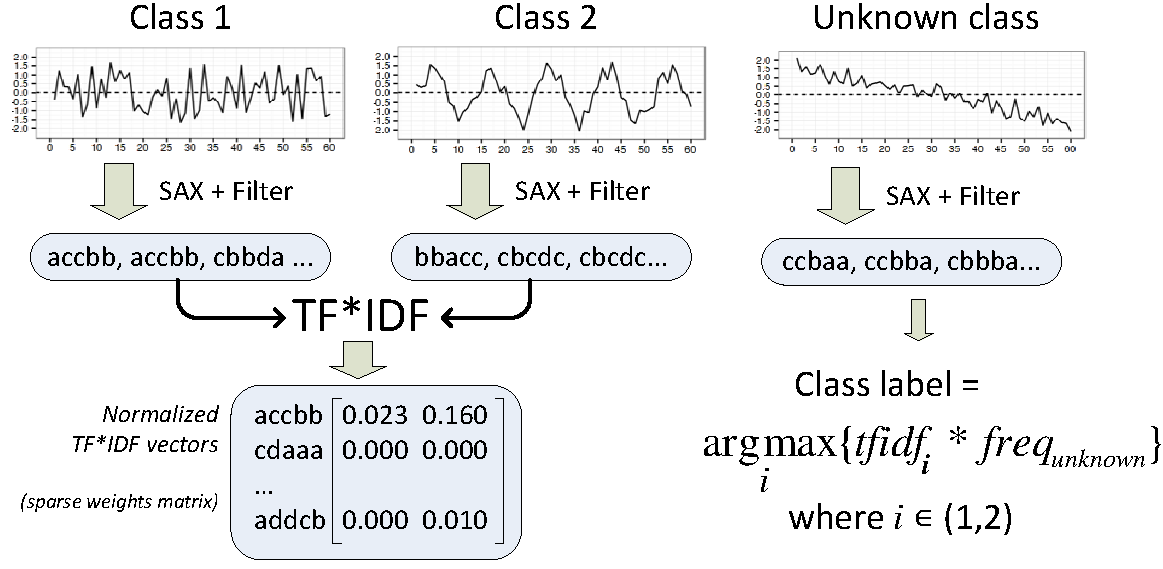
\includegraphics[width=115mm]{figures/overview.eps}
   \caption{A simplified overview of SAX-VSM algorithm: at first, labeled series are converted into
bags of words using SAX; 
secondly, \textit{tf$\ast$idf} statistics for two-bags corpus is computed, resulting in one weights
vectors for each class.
Unknown series are classified by the label of the weight vector having the minimal angle (maximal
cosine value) with the words frequency vector built by SAX application to the unknown series.}
   \label{fig:overview}
\end{figure}

\subsection{Classifier training phase}
In order to employ Information Retrieval techniques, we transform all labeled time-series instances
from each of training classes into the single bag of words. For this, our algorithm converts a real
valued time series into SAX string representation configured by four parameters: the sliding window
length (\textit{W}), the number of PAA frames per window (\textit{P}), the SAX alphabet size
(\textit{A}), and by the complexity reduction strategy (\textit{S}). 
As we mentioned, each of the extracted with sliding window subseries is normalized by energy before
being processed with PAA \cite{goldin_kanellakis}. If, however, the standard deviation of the
time-series values is below a fixed epsilon threshold, we do not apply this normalization.

By applying this procedure to all $N$ training classes, we build a corpus of $N$ bags, which, in
turn, we process with \textit{tf$\ast$idf}. This provides $N$ real-valued vectors of equal
length, each of which represents one of the training classes classes. These vectors are normalized
by Cosine normalization procedure and used in the classification phase.

\subsection{Classification phase}
Similarly to training phase, in order to classify an unknown time-series, we transform it into the
terms vector using the same SAX parameters which we have used in the training phase. 
Then, we compute cosine values between this terms vector and vectors which represent $N$ known
classes. The series is assigned to the class whose vector yields the maximal cosine similarity
value.

\subsection{SAX Numerosity reduction}
As noted in \cite{sax}, given a character subsequence $S_{i}$ extracted by the use of sliding
window and SAX, it is very likely, that $S_{i}$ is very similar to its neighboring subsequences,
$S_{i−1}$ and $S_{i+1}$ (i.e. those that start one point to the left, and one point to the right of
$S_{i}$), especially if $S_{i}$is in the smooth region of the time series. This phenomena results in
mapping of multiple consecutive subsequences to the same string. The authors called these
subsequences as ``trivial matches'' of $S_{i}$, and suggested to avoid their over-counting
introducing a ``numerosity reduction technique'' by keeping only the first occurrence of $S_{i}$. 

While the inclusion of numerosity reduction into workflow seems to be reasonable for SAX
applications, namely motif and discords finding, we found, that SAX-VSM classifier performs
significantly better without it on thirty one dataset representing a variety of real-life
applications \cite{jmotif}.
We believe, that in SAX-VSM the over-counting effect is significantly mediated by
\textit{tf$\ast$idf} statistics, which reduces the effect of raw counts. Also, this conclusion is
similar to one articulated in \cite{bag_patterns}.

Nevertheless, our SVM-SAX implementation \cite{jmotif}, provides two strategies for numerosity
reduction. First, called $CLASSIC$ is based on the string distance function $MINDIST$ proposed
in \cite{streaming_sax}. Second strategy, called $EXACT$ is based on the Hamming distance
\cite{hamming}. 

\subsection{SAX Parameters selection} \label{section-direct}
We use a common cross-validation scheme while exploring possible parameters space. 
In order to accelerate the search for optimal set, 
we utilize DIRECT (DIviding RECTangles) algorithm, which 
was introduced by Jones et al. \cite{direct-original}. This optimization scheme 
designed to search for global minima of a real valued function over a bound-constrained domain. 
In our implementation we use rounding of parameters by nearest integer function.

The algorithm iteratively performs two procedures - partitioning the search domain, 
and identifying potentially optimal hyperrectangles (i.e., having potential to contain good
solutions). 
It begins by scaling the search domain to a n-dimentional unit hypercube which is considered 
as potentially optimal. The error function is then evaluated at the center of this hypercube. Next, 
other points are created at one-third of the distance from the center in all coordinate directions. 
The hypercube is then divided into smaller rectangles which are identified by their center point 
and their error function value. This procedure continues interactively until error function
converges.
For brevity, we omit the detailed explanation of the algorithm, and refer the 
interested reader to \cite{direct} for additional details about our implementation.

\begin{figure}[tbp]
   \centering
   \includegraphics[width=120mm]{figures/figure_direct.eps}
   \caption{Illustration of parameters
optimization with DIRECT algorithm for \textit{SyntheticControl} dataset. Left panel shows
all points sampled by DIRECT in the space $PAA*Window*Alphabet$ - red points correspond to high
error values in cross-validation experiments, while green points correspond to low error values;
note the green points concentration at $W$=42.\\ 
Middle panel shows the error-rate heatmap when the sliding window size is fixed to 42, this figure
was obtained by complete scan of all 432 points.\\ 
Right panel shows the optimized by DIRECT sampling,
optimal solution ($W$=42,$P$=8,$A$=4) was found by sampling of 43 points.}
   \label{fig:direct-sampling}
\end{figure}
   
\subsection{Intuition behind SAX-VSM}
First of all, by using sliding window and by combining all of observed in the class SAX words into
a 
single bag, SAX-VSM manages to exhaustively capture an intraclass variability at the sliding window 
length granularity. Intuitively, this improves the algorithm's selectivity by facilitating a proper 
classification of time series which possess low similarity to labeled series at the full length, 
but embed characteristic to the class features.

Secondly, the \textit{tf$\ast$idf} statistics naturally ``highlights'' the terms unique to the
class by assigning them higher weights, while terms observed in a number of classes are assigned
weights inversely proportional to their interclass presence frequency. This weighting scheme
naturally improves the selectivity of classification by  lowering the contribution of ``confusive''
multi-class terms, and  increasing  the contribution  of  class' ``defining'' terms to the final
cosine value.   
   
\section{Results}
We have proposed a novel algorithm for time series classification based on the SAX
representation of time series and Vector space model called SAX-VSM. Here we present a range of
experiments assessing its performance for classification and clustering.

\begin{figure}[t]
   \centering
   \includegraphics[width=115mm]{figures/precision-runtime.ps}
   \caption{Comparison of precision and runtime of SAX-VSM and 1NN Euclidean classifier on
CBF data: SAX-VSM performs much better with limited amount of training samples at relatively high
cost while with the growth of labeled data, both classifiers demonstrate similar performance.
SAX-VSM is much faster in classification and comparable with 1NN classifier cost when training time
is accounted.}
   \label{fig:precision-runtime}
\end{figure}

\subsection{Classification performance}
To evaluate our approach, we selected thirty one data set. Majority of the data sets was taken 
from the UCR time series repository \cite{ucr}, the Ford data was originally used in a competition
at the IEEE World Congress on Computational Intelligence \cite{ford}, the Electrical Devices
dataset was downloaded from supporting website for \cite{bagnal}.

Overall, SAX-VSM classification performance found to be at the level of best
performing 1-NN classifiers (whether based on Euclidean distance, DTW, or SAX), shapelet tree, or a
shapelet-based SVM. This result is not surprising taking in account ``No Free Lunch theorems''
\cite{nfl}, which assert, that there will not be a single dominant classifier for all TSC problems.

For synthetic data sets, it is possible to create as many instances as one need for experimentation.
We used CBF data set \cite{cbf} to investigate the performance of SAX-VSM and 1NN Euclidean
classifier on increasingly large training data sets of size 10, 50, 125, ..., 1000, and a fixed test
dataset of 10000 instances. For small training data sets, SAX-VSM is significantly more accurate
than 1NN Euclidean classifier, however, by the time we have more than 500 time series in
our training set, there was no statistically significant difference in accuracy. 
As per classification runtime cost, SAX-VSM was found more expensive than 1NN Euclidean classifier
when training set is small mostly due to the training cost. For the large training sets, there was
no significant difference in the overall runtime speed for both classifiers. 
However, SAX-VSM allows to perform training offline and load \textit{tf$\ast$idf} weights vector as
needed. If this option utilized, the classification time cost is always significantly less than that
of 1NN Euclidean classifier \ref{fig:precision-runtime}.

Table \ref{perf_table} includes twelve known datasets, for which we were able to recover performance
metrics for four classifiers: 1NN classifiers based on Euclidean distance and DTW, and
recently proposed classifiers based on shapelet decision trees \cite{shapelet} \cite{logical}, and
the shapelet transform \cite{bagnal}. These datasets represents a variety of possible applications. 

We used train/test split and all reported
results are testing accuracy. All SAX parsing parameters and the bag construction strategy were
found exclusively on a training set in cross-validation experiments as
explained in Section \ref{section-direct}. The test set was used only once with the final set of
parameters. Our algorithm implementation is publicly available at \cite{jmotif}.

{\scriptsize
\begin{table}[t]%
\caption{\bf Classifiers error rates comparison.}
 \label{perf_table}
\centering
\begin{tabularx}{\linewidth}{@{} l *5X @{}}\toprule[1.5pt]
\bf Dataset &\bf 1NN-Euclidean &\bf 1NN-DTW &\bf Shapelet Tree &\bf  Shapelet SVM &\bf 
SAX-VSM\\\midrule
%\bf Variable Name & \bf Regression 1 & \bf Mean & \bf Std. Dev & \bf Min & \bf Max\\\midrule
%text        &  text     & text      &  text     &  text     &text\\
%\bottomrule[1.25pt]
%\end {tabularx}
%\begin{tabular}[h]{  l | c | c | c | c |  c  }
%\hline
%Dataset           & 1NN-Euclidean  & 1NN-DTW       & Shapelet Tree & Shapelet SVM & SAX-VSM \\
%\hline
SyntheticControl  & 0.120   & \textbf{0.007}  & 0.057     & 0.127            & 0.010 \\
Adiac             & 0.389   & 0.396           & 0.700        & 0.762         & \textbf{0.381}\\
Beef              & 0.467   & 0.467           & 0.500        & 0.133         & \textbf{0.033}\\
ChlorineConcentration  & 0.350 & 0.350        & 0.412        & 0.439         & \textbf{0.332} \\
Coffee            & 0.250   & 0.180           & 0.036     & \textbf{0.0}     & \textbf{0.0} \\
ECG               & 0.120   & 0.230           & 0.149     & \textbf{0.007}   & 0.09 \\
ElectricDevices   & 0.913   & 0.913           & 0.451     & 0.756            & \textbf{0.329} \\
FaceFour          & 0.216   & 0.170           & 0.159     & 0.023            & \textbf{0.0} \\
Gun Point         & 0.087   & 0.093           & 0.107     & \textbf{0.0}     & 0.007 \\
Lightning7        & 0.425   & \textbf{0.274}  & 0.507     & 0.314            & 0.301 \\
SonyAIBO          & 0.306   & 0.274           & 0.155     & \textbf{0.133}   & 0.176 \\
Trace             & 0.240   & \textbf{0.0}    & 0.020     & 0.020            & \textbf{0.0} \\
\bottomrule[1.25pt]
\end{tabularx}
\end{table}
%\hline
%\end{tabular}
}

\subsection{Robustness to noise}
In our experimentation we observed, that the dimension of \textit{tf$\ast$idf} weights vectors 
grows following the grows of the training set size. While it grows rapidly at the beginning, once
the dictionary is saturated, growth tend to slow down (left panel of Figure \ref{fig:corrupted}). 
Nevertheless, by adjusting alphabet and PAA sizes it is possible to keep the number of terms
significantly large. 

This observation and the fact that terms are originating from the full span of time series prompted
the idea that SAX-VSM classifier might be robust to the loss of signal in unlabeled
series. Intuitevely, if some of the class representative terms will be lost, the cosine
similarity might not degrade significantly enough to cause missclassification.

\begin{figure}[H]
   \centering
   \includegraphics[width=115mm]{figures/corrupted.eps}
   \caption{Left panel: Illustration of terms growth for CBF corpus and individual classes.
Right panel: illustration of 1-NN Euclidean and SAX-VSM performance on corrupted data.}
   \label{fig:corrupted}
\end{figure}

While we plan to perform more exploration, at this point we found, that by randomly replacing up
to 30\% span of CBF test series with random noise, SAX-VSM performing consistently better
than 1NN Euclidean classifier as shown at the right panel of Figure \ref{fig:corrupted}
\todo{need to exercise this point further}

\subsection{Exploratory data analysis}
While classification results reported in previous section show that SAX-VSM classifier
has very good potential, one of the strengths of using it as a classification tool is that
it facilitates a superior level of interpretation when compared with other techniques. 

Previously, with a number of examples it was shown in original work on shapelets \cite{shapelet}
that the resulting decision trees provide interpretable classification and an insight into the data
specific features. In successive work \cite{bagnal} based on shapelets, it was shown that
discovery of multiple shapelets provides even better intuition into interpretability of
classification. However, the authors noted, that a time cost of multiple shapelets discovery
could be significant. Contrary, SAX-VSM provides numerous weighted patterns at no time cost
allowing further insight into interpretability.

\subsection{Gun Point data}
Following mentioned shapelet-based work \cite{shapelet} and\cite{bagnal}, we used a well-studied
\textit{GunPoint} dataset to explore the interpretability of classification results.
The data set contains time series of an actor performing the motion of drawing a gun
(\textit{Gun}), and pretending of drawing a gun (\textit{Point}), and the classification problem is
to determine whether or not she were holding a gun or imitated the action.

Similarly to reported results, SAX-VSM was able to capture both features which are distinguishing
problem's classes as shown at the Figure \ref{fig:shapelet-like-patterns}. The most weighted SAX
pattern in \textit{Gun} class situated at the beginning of time series and corresponds to the subtle
extra movements required to lift and aim the prop. 
The most weighted SAX pattern in \textit{Point} class found at the ending of time series and
corresponds to to the ``overshoot'' phenomena which is causing the dip in the time
series. 
The second to best pattern in \textit{Point} confirms class' difference in the propless hand
raise. 
Our findings align exactly with all previously published work \cite{shapelet} \cite{bagnal}.

\begin{figure}[t]
   \centering
   \includegraphics[width=110mm]{figures/shapelet-patterns.ps}
   \caption{Examples of two best weighted sub-series from each class of \textit{GunPoint} dataset. 
   Note, the upward arm motion is more ``important'' for a \textit{Gun} class, whether downward arm
motion for \textit{Point} class. These result align with previous work \cite{shapelet} and
\cite{bagnal} in which similar locations were reported. Second to best patterns outline the the
differences in aiming (\textit{Gun}) and smooth ``propless'' hand movement in \textit{Point} class.
   }
   \label{fig:shapelet-like-patterns}
\end{figure}

\subsection{OSU Leaf data}
According to the original data source, Ashid Grandhi \cite{osuleaf}, with the current growth of
digitized data, there is a huge demand for automatic management and retrieval of various images. The
\textit{OSULeaf} dataset consist of curves obtained by color image segmentation and boundary
extraction (in the anti-clockwise direction) from digitized leaf images of six classes: \textit{Acer
Circinatum, Acer Glabrum, Acer Macrophyllum, Acer Negundo, Quercus Garryana and Quercus Kelloggii}.
While the authors of the original work were able to solve the problem of leaf boundary curves
classification by use of DTW achieving 60\% accuracy, DTW, as we pointed above, provides a very
little information about why it succeeds of fails. 

\begin{figure}[t]
   \centering
   \includegraphics[width=115mm]{figures/AcerCircunatum.eps}
   \caption{Illustration of the best discriminating patterns found by SAX-VSM for
\textit{OSULeaf dataset}. These patterns align with well known in botany discrimination techniques
by lobe shapes, serrations, and the leaf tip type.}
   \label{fig:shapelet-acer-patterns}
\end{figure}

In contrast, SAX-VSM application yielded a set of class-specific characteristic patterns for each of
six leafs classes from the \textit{OSULeaf} dataset which closely match known techniques of leafs
classification based on leaf shape and margin \cite{dirr}. These features include the slightly
lobed shape and acute tips of Acer Circinatum leafs, serrated blade of Acer Glabrum leafs,
the accuminate tip and characteristic serration of in Acer Macrophyllum leafs, pinnately compound
leafs arrangement of Acer Negundo, the incised leaf margin of Quercus Kelloggii, and a lobed leaf
structure of Quercus Garryana. Figure \ref{fig:shapelet-acer-patterns} shows three of these classes
along with their highlighted features at leafs images and within corresponding class time series.

Further, we found, that in the \textit{Coffee} spectrogram dataset SAX-VSM highlighted spectrogram
intervals corresponding to Caffeine and Chlorogenic acid - two chemical compounds responsible for
the differences in coffee flavor, which also aligns with previosly reported findings \cite{coffee}

\section{Clustering}
Clustering is a common tool used for data visualization, exploration, and partitioning. 
In addition, clustering serves as a subroutine in many others data mining algorithms.

\subsection{Hierarchical clustering}
We applied hierarchical clustering procedure to \textit{SyntheticControl} dataset clustering
eighteen time series in total, three from each of the classes \textit{increasing trend, decreasing
trend, upward shift, downward shift, periodic, and normal}. Figure \ref{fig:hc} shows
clustering. Obviously, it shows superiority of SAX-SVM distance performance over Euclidean in
hierarchical clustering.

\begin{figure}[t]
   \centering
   \includegraphics[width=115mm]{figures/clustering.eps}
   \caption{A comparison of hierarchical clustering application to \textit{SyntheticControl}
dataset. Complete linkage was used for these plots.
   }
   \label{fig:hc}
\end{figure}

\subsection{kMeans clustering}
Again, reflecting concepts of IR field, kMeans clustering based on SAX-VSM approach effectively
is the spherical kMeans approach, which has a number of known advantages. First of all, it can be
parallelized for efficient computation \cite{modha}, and usually converges quickly. Furthermore,
computed centroids generalize cluster members and can be used as a ``model'' to classify future 
time series.

\section{Conclusion}
In our opinion, the superior classification performance of our approach is based on 
a number of factors. 
First of all, our approach is very different in nature from those 
based on convenient distance measures such as Euclidean distance or DTW - to some 
extent we do not pay attention to ordering of time points outside of sliding window. 
Surely, overlapping windows do carry information about initial ordering, but this 
is fading away along the steps of our algorithm.
Secondly, we are able to efficiently tolerate noise by leveraging agglomeration 
and mediation with PAA. 
Thirdly, the SAX alphabet cuts provide flexible boundaries for capturing similar 
sub-series. 
And finally, Vector space model and textit{tf$\ast$idf} statistics provide us 
with efficient discrimination and measurement toolkit: the tf part of the weighting scheme
captures the frequency of observed feqtures within the class, while the idf part 
captures the feature informativeness (features that appear in many classes 
are less informative than those that appear rarely)

\subsection{Limitations}
Currently, while SAX and Vector Space model naturally support extraction and processing of multiple
word lengths in the same classifier, our implementation lacks this capacity. Certainly this is a
major limitation since shapelet-based techniques \cite{bagnal} not only provide such a feature
but prove its superior performance.

While DIRECT optimization provides satisfiable performance, it is designed for function
defined on real values, whether SAX parameters defined only on integer domain. In our
experimentation we observed DIRECT redundantly sampling same locations due to the rounding scheme
we use. More appropriate optimization scheme is needed.


\section{Future directions}
Note, that just as in Linguistics, such a corpus could be built from bags of SAX words obtained with
different parameters, or, moreover, by parsing every single series by more than once. This,
potentially, not only improves performance of our technique, but also facilitates multivariate
series classification.

%
% ---- Bibliography ----
%
\begin{thebibliography}{5}
\bibliographystyle{splncs}
%

%1
\bibitem {1NN}
Xi, X., Keogh, E., Shelton, C., Wei, L., Ratanamahatana, C.A. 2006. 
Fast time series classification using numerosity reduction. 
In Proc of the 23rd international conference on Machine learning (ICML '06). 1033--1040.

%2
\bibitem {DFT}
Agrawal, R., Faloutsos, C., Swami, A. 1993.
Efficient Similarity Search In Sequence Databases.
In Proc FODO '93. 69-84.

%3
\bibitem {spade}
Chen, Y., Nascimento, M. A., Ooi, B. C., Tung, A. K. H.:
Spade: On shape-based pattern detection in streaming time series. 
In Proc. of the IEEE 23rd International Conference on Data Engineering, 2007, pp. 786–795.

%4
\bibitem {benchmark}
Keogh, E., Kasetty S. 
On the need for Time Series Data Mining Benchmarks: a survey and empirical demonstration.
Proc. ACM KDD 2002, pp. 102-111.

%5
\bibitem {indexing}
Keogh, E. 2002. 
Exact indexing of dynamic time warping. 
In Proc of the 28th international conference on Very Large Data Bases (VLDB '02). 406-417.

%6
\bibitem {shapelet}
Ye, L., Keogh, E.:
Time series shapelets: a new primitive for data mining. 2009.
In Proc of the 15th ACM SIGKDD international conference on Knowledge discovery and data
mining. 947--956.

%7
\bibitem {logical}
Mueen, A., Keogh, E., Young, N. 2011.
Logical-shapelets: an expressive primitive for time series classification.
In Proc of the 17th ACM SIGKDD international conference on Knowledge discovery and data
mining. 1154--1162.

%8
\bibitem {bagnal}
Lines, J., Davis, L.M., Hills, J., Bagnall, A. 2012.
A shapelet transform for time series classification. 
In Proc 18th ACM SIGKDD KDD '12. 289-297.

%9
\bibitem {comparison}
Ding, H., Trajcevski, G., Scheuermann, P., Wang, X., and Keogh, E. 2008.
Querying and Mining of Time Series Data: Experimental Comparison of Representations and Distance
Measures. 
In Proc of the 34th VLDB. 1542–1552, 2008

%10
\bibitem {classifiers}
Salzberg, S.L. 1997.
On comparing classifiers: Pitfalls to avoid and a recommended approach. 
Data Mining and Knowledge Discovery, 1, 317–328.

%11
\bibitem {sax}
Lin, J., Keogh, E., Wei, L., Lonardi, S. 2007.
Experiencing SAX: a novel symbolic representation of time series.
Data Mining and Knowledge Discovery, 107--144.

%12
\bibitem {salton}
Salton, G., Wong, A., Yang., C.S. 1975.
A vector space model for automatic indexing. 
Commun. ACM 18, 11, 613--620.

%13
\bibitem {direct}
Björkman, M., Holmström, K.
Global Optimization Using the DIRECT Algorithm in Matlab.
Advanced Modeling and Optimization, 1999, 1(2),17-37

%14
\bibitem {hot_sax}
Keogh, E., Lin, J., Fu, A. 2005.
HOT SAX: Efficiently Finding the Most Unusual Time Series Subsequence. 
In Proc ICDM '05. 226-233.

%15
\bibitem {fast-shapelets}
Fast-Shapelets: A Scalable Algorithm for Discovering Time Series Shapelets
Rakthanamanon, T., Keogh, E.
In proc of SIAM Conference on Data Mining (SDM13).

%16
\bibitem {goldin_kanellakis}
D.Q., Kanellakis, P.C., 1995.
On Similarity Queries for Time-Series Data: Constraint Specification and Implementation. 
In Proc CP '95. 137-153.

%17
\bibitem {paa}
Keogh, E., Pazzani, M.J. 2000.
A Simple Dimensionality Reduction Technique for Fast Similarity Search in Large Time Series
Databases. 
In Proc PADKK '00. 122-133.

%18
\bibitem {larsen_marx}
Larsen, Richard J. and Marx, Morris L. 2000. 
An Introduction to Mathematical Statistics and Its Applications (3rd Edition).
Prentice Hall.

%19
\bibitem {streaming_sax}
Lin, J., Keogh, E., Lonardi, S., Chiu, B. 2003.
A symbolic representation of time series, with implications for streaming algorithms. 
In Proc 8th ACM SIGMOD workshop DMKD '03. 2-11.

%20
\bibitem {bag_patterns}
Lin, J., Khade, R., Li, Y. 2012.
Rotation-invariant similarity in time series using bag-of-patterns representation. 
J. Intell. Inf. Syst. 39, 2 , 287-315.

%21
\bibitem {jmotif}
Paper Authors. 
Accompanying information for this paper. 
\url{https://code.google.com/p/jmotif/}

%22
\bibitem {hamming}
Hamming, R.W. 1950.
Error detecting and error correcting codes. 
Bell System Technical Journal 29, pp. 147--160

%23
\bibitem {direct-original}
Jones, D.R., Perttunen, C.D., Stuckman, B.E.:
Lipschitzian Optimization without Lipschitz Constant.
Journal of Oprtimization Theory and Applications, 79 (1), 1993.

%24
\bibitem {ucr}
Keogh, E., Zhu, Q., Hu, B., Hao. Y.,  Xi, X., Wei, L., Ratanamahatana, C. A. 2011.
The UCR Time Series Classification/Clustering Homepage:
\url{http://www.cs.ucr.edu/~eamonn/time_series_data/}

%25
\bibitem {ford}
WCCI, Ford classification challenge, \url{http://home.comcast.net/~nn_classification/}

%26
\bibitem {nfl}
Wolpert D. H., Macready, W. G. 1997
No free lunch theorems for optimization.
IEEE Trans. on Evo. Comp. 1 no. 1, pp. 67--82.

%27
\bibitem {cbf}
P. Geurts. 2002.
Contributions to Decision Tree Induction: bias/variance tradeoff and time series classification.
PhD thesis, University of Lige, Belgium.

%28
\bibitem {osuleaf}
Gandhi, A. 2002.
Content-Based Image Retrieval: Plant Species Identification. 
Master thesis, Oregon State University.

%29
\bibitem {dirr}
Dirr, M. A. 2013.
Manual of Woody Landscape Plants: Their Identification, Ornamental Characteristics,
Culture, Propogation and Uses.
Stipes Pub Llc, ed. 6 Revised.

%30
\bibitem {coffee}
Briandet, R., Kemsley, E.K., Wilson, R.H. 1996
Discrimination of Arabica and Robusta in Instant Coffee by Fourier Transform Infrared Spectroscopy
and Chemometrics.
J. Agric. Food Chem. 1996, 44, 170−174

%31
\bibitem {modha}
Dhillon, S.I., Modha, D.S. 1996., May 2002
A Data-Clustering Algorithm on Distributed Memory Multiprocessors. 
In Proc Workshop on Large-Scale Parallel KDD Systems, SIGKDD, 245-260.

\end{thebibliography}

%\clearpage
%\addtocmark[2]{Author Index} % additional numbered TOC entry
%\renewcommand{\indexname}{Author Index}
%\printindex
%\clearpage
%\addtocmark[2]{Subject Index} % additional numbered TOC entry
%\markboth{Subject Index}{Subject Index}
%\renewcommand{\indexname}{Subject Index}
%\input{subjidx.ind}
\end{document}
